% changing latex compiler for use with external fonts
% !TEX TS-program = xelatex
\documentclass[12pt]{report}

\usepackage[utf8]{inputenc} % Required for inputting international characters
\usepackage[T1]{fontenc} % Output font encoding for international characters
\usepackage{graphicx} % images
\usepackage{fancyhdr} % headers and footers
\usepackage{parskip} % paragraph
\usepackage{geometry} % shapes
\usepackage{hyperref} % Links
\usepackage{pdflscape} % making a page landscape
\usepackage{listings} % writing code snippets
\usepackage{fancyvrb} % extra functionality for verbatim
% \usepackage{fontspec} % changing fonts
\usepackage[]{microtype} %

% \usepackage{microtype} % used for formatting nicely and getting rid of hbox badness
% \usepackage{natbib}
\usepackage{float} % to place figures in place

\graphicspath{{../images/}}

\renewcommand{\bibname}{References}
\renewcommand{\baselinestretch}{1.5}

% font family change
% \setmainfont{Times New Roman}



\bibliographystyle{unsrtnat}
\graphicspath{{../images/}}

% setup the styling for code snippets
\lstset{
  basicstyle=\ttfamily,
  columns=fullflexible,
  frame=single,
  breaklines=true,
  postbreak=\mbox{\textcolor{red}{$\hookrightarrow$}\space},
}



% hyperlink setup
\hypersetup{
    colorlinks,
    citecolor=black,
    filecolor=black,
    linkcolor=black,
    urlcolor=black
}

% margins and page size
\geometry{
a4paper,
left=25mm,
top=25mm,
right=25mm,
bottom=25mm
}

\begin{document}

\begin{titlepage}
\center
{\huge\bfseries Report}  
\end{titlepage}

\tableofcontents

\chapter{Abstract}
This project aim is to create a Souls-Like game with an AI system that allows for in-fighting between creatures based on a food chain. I researched different AI techniques to pull this off and landed on GOAP - Goal Oriented Action Planning - as the system I would use in this game.
\chapter{Introduction}
\chapter{Output Summary}
\chapter{Literature Review}
My project focuses on creating a game in the souls-like genre where the enemies act in an eco-system where there is a food-chain hierarchy in which they can fight each other.

An intricate in-fighting system between multiple different AI agents is what I will be focusing on. One of the early examples of in-fighting was seen in the original Doom (1993)\cite{doom93}, where if an enemy-A got attacked by enemy-B, enemy-A will change it's target from player to enemy-B, this is a very simple system but offers many different gameplay opportunities, many levels were crafted with this in mind where the players would have to manipulate the AI by luring one enemy into another's line of fire.
This idea was later expanded by Ubisoft in their later Far Cry games where different clans can combat each other in random events, and animals can also combat each other, combining these together, there a re many random events where animals attack enemies that are already mid combat between you and another clan. In Far Cry Primal they expanded the animal system so that you could tame any animal in the world and make them your companion in gameplay.

This sort of systemic game design is created by making the different game systems aware of each other, and this inturn invites the player to use their creativity to make plans on how to execute their goals and creating unique experiences. This type of gameplay has been coined as emergent gameplay where complex systems \textit{emerge} from the interaction on relatively simple game mechanics.\cite{emergentGameplay}

There are different types of AI techniques that I could use, the following are the ones that I have looked into: Finite State Machines, Behaviour Trees, Goal Oriented Action Planning and Utility Based AI.

Finite state machines are the most rudimentary AI system, it is a system that I had implemented in my Advanced Games Tech Project, these are very easy and quick to implement for a simple AI system however it does not suit the complex AI behaviours I would like to build as when adding more complexity to a state machine, the "program flow becomes much more difficult to understand and creates a debugging nightmare"\cite{gameAiByExample}.

Behaviour Trees were popularised by Halo 2\cite{halo2} and are now the most common AI technique used in modern games, this is due to there being a streamlined flow/logic to the readability of the AI, this makes it easier to expand while keeping debugging simple. The design is built using nodes as modules, allowing nodes to be reused with minimal effort. There is also a 'blackboard' where shared knowledge is kept which the AI uses to make 'smarter' decisions while keeping memory usage to a minimum. This all happens while keeping a low computational overhead if implemented correctly. \cite{behaviourTrees}

Goal Oriented Action Planning (GOAP) was originally implemented in a game in F.E.A.R (First Encounter Assault Recon) by Jeff Orkin \cite{goap}. It is a system that is made up of many actions, these actions comprise of objects, preconditions and effects; an agent will decide on an action to execute based on their current situation and then work backwards through the preconditions to create an efficient plan of executing the actions. This is done using an A* path finding algorithm, the actions have different weightings based on how easy they are to execute from the current state of the agent. This system can be very easy to scale if the ground work is set up properly as all would have to be done is add more actions in. Similar to behaviour trees (BT), a blackboard is used to store shared data which the AI can use to make decisions. This system can have performance issues, as goals and plans will have to be calculated for every active agent very frequently, so increasing the number of agents in the scene will have a performance hit. This was an issue when F.E.A.R came out as the rats in the game used the same AI system as the enemies, and once a rat had spawn, it would not be destroyed, and this would accumulate over a long play session and cause performance issues. This system can create novel AI behaviour which isn't seen easily in BT and FSM AI design. This is the system I would like to implement as it would be easier to create AI that seems to behave 'organically' like they do in F.E.A.R.. \cite{goapTommyTompson} An example of this is given in Jeff Orkin's 2003 paper on the subject of applying GOAP\cite{applyingGoap}, he talks about a character X running out of ammunition in their weapon, given that their goal is still to eliminate the enemy, the planner will find another way of doing that - in the example, there is a laser that can be activated by both player and enemies - the planner will now find a combination of actions to execute in a particular order for the enemy to activate the laser to eliminate the player. This is a novel idea that the planner came up with by using what was in the environment, behaviour like this would be missed in games using behaviour trees as that particular course of action was not added into the tree.
%might not need to cite tommy thompson

\chapter{Method}
% methodology then tools used
\section{Software Design Methodology}
% IE. Agile or something

The AI system is based around GOAP which works really well as a modular system that can bring about novel ideas by agents.

\section{Tools}
%tools
% need to add
% - Audio Tool
% - UML tool
% - evaluation tool

\subsection{Unity (Game Engine)}
Unity was chosen as the game engine over Unreal Engine as I had some prior (albeit minimal) experience in using it; Unity used C\# for scripting which is, for me, a simpler language to write in over C++, even though I have used C++ more extensively over the past year in various projects. Unity also had better performance on the hardware and operating system I would be using for this project, while being smaller in file size.

As mentioned in my PDD, Unity has an extensive amount documentation available on their website which is easy to understand, they also have a forum site where there is a very active community in helping new-comers with any issues they face; as well as this, there are plenty of tutorials about Unity on their own website and on YouTube.

There is also an asset store built into Unity with many paid and free assets, ranging from scripts, models, materials, shaders, physics systems and more.

All of this combined, it was very difficult for me to not choose Unity as the Game Engine for my project.

\subsection{JetBrains Rider (IDE)}
JetBrains Rider was my choice of IDE as I have been using JetBrains products since the Programming in Java module in the first year, and I feel they provide a very good set of refactoring and debugging tools with a good amount of community made extensions for the program. Rider was created as a .NET IDE, and now has native Unity support, which is perfect for use with Unity.

My other option was Microsoft's Visual Studio, which I had used in the second and third year Games Tech modules. After using it, I did not like it much and had installed the ReSharper plugin by JetBrains, which brought some of the functionality from JetBrains IDEs. Given that JetBrains have their own IDE for Unity, I decided to go with that over Visual Studio.

\subsection{GitHub}
I used GitHub as my version control and backup system as I am very familiar with it. I have used it extensively over my time at the university.

\subsection{Blender}
I used Blender as my 3D program of choice as it is very intuitive to learn and very simple to use. It is also free and open source leading to very many tutorials for it along with great documentation. It has support for opening most 3D filetypes which is good for me as I will be getting assets from different locations; if there is a filetype that is not supported, then there is bound to be an extension for it, due to the many community mad extensions available.

\subsection{Adobe Photoshop}
This is my image editor of choice as I am very well versed in it and have been using it over the past 6 years and professionally for the past 2 years.

\subsection{Adobe Illustrator}
Adobe Illustrator was the choice of vector editor used to design any graphical elements that cannot be created in Unity's GUI system and used to design the GUI in the planning phase. 

\subsection{diagrams.net}
Diagrams.net (formally known as draw.io) was used as the tool to create UML diagrams as it is a lightweight web-application providing all the necessary features and flexibility. The feature that came in most useful was the integration with github; I was able to save my diagrams and version them directly in the same repository.

\section{Programming Patterns}
The programming paradigm used was based around an Entity Component System (ECS) design where there are Entities in the world (the game objects) that are built up of components.
Games in Unity are built around this paradigm, preferring a system of composition over inheritance. It allows for greater flexibility as unlike inheritance where you 'inherit' all features at once, you build the game object using components(C\# classes) that you build that are fulfil a very specific purpose. This leads to code being very modular and less coupled, leading to faster development as changing one component will not have a ripple effect on others. 
The following shows the flaws with inheritance for development\cite{CompOverInherit}:
\begin{lstlisting}
ROBOT // parent class
    .drive()
        MurderRobot // inherited class
            .kill()
        
        CleaningRobot // inherited class
            .clean()

ANIMAL // parent class
    .poop()
        Dog // inherited class
            .bark()

        Cat // inherited class
            .meow()
\end{lstlisting}
Now the above works great and would serve you through most of the project, but the problem arises if down the line you would like to create a \lstinline{MurderRobotDog} that can \lstinline{drive()}, \lstinline{kill()} and \lstinline{bark()}, however being a robot it cannot  \lstinline{poop()}. There are only a few solutions around this, 

1. you do a multiple inheritance and accept that you will have extra unnecessary functionality, 

2. you create a new Robot inherited from  \lstinline{MurderRobot} and duplicate the  \lstinline{bark()} functionality, 

3. you create a superclass of both that has a  \lstinline{bark()} functionality, this leads to unnecessary functionality in most instances. 

To solve this problem you will have to take time out from creating new features and refactor the codebase to work within good coding standards\cite{codingPractices}.

If designed using composition, it would look like the following \cite{CompOverInherit}:
\begin{Verbatim}[frame=single]
ENTITIES          COMPONENTS (in the form of classes)
Dog             : pooper + barker
Cat             : pooper + meower
CleaningRobot   : driver + cleaner
MurderRobot     : driver + killer
MurderRobotDog  : driver + killer + barker
\end{Verbatim}
This provides you with the most flexibility to create whatever type of game object you would like while being loosely coupled and avoiding duplication.

Inheritance was not abandoned and was used in the places necessary, like creating the \\ \lstinline{BaseAIGoap} class. %\\ to fix overfull h-box

A game object with components can be saved as a prefab, which can then be reused, an example would be creating an enemy prefab, and then creating an enemy spawner that loads copies of that prefab into the scene.

\section{Software Design}

\subsection{Modelling Actions}
The actions for the AI agents were modelled before modelling the class diagrams. 

\subsection{Class Diagrams}
Class diagrams are a great to draw out a visual plan of what the system will look like. As I am using an ECS form of design, the class diagram will mainly consists of many classes with compositional relationships.

\subsection{User Interface (UI)}
Adobe Illustrator was used to draft out the user interface. Some UI elements will exist within the 3D world space, these are called spacial UI elements; these types of UI elements allow the player to receive the information they require without taking up much space on the orthographic canvas where more player related statistics can go.\cite{UIChoices}

\subsection{Misc}

% \section{Project Objectives}
% The Project objectives can be found in the Project Definition Document (PDD) in Appendix 1
% \subsection{Minimum Viable Product}
% \subsection{Creatures}


\chapter{Result}
% \section{Milestone 1}


\section{Minimum Viable Product}

\subsection{Modelling the Actions}
The AI system was abstracted into the different actions the AI will be performing and the goals it will use to plan out the course of action. Seen in the figure below is the simple set of actions and goals sufficient for the first build and will have the ground work to expand upon the next build. The food ready goal and precondition for eat food will be used to add the attacks for the creature's higher in the food chain, like the Lizard, as they should only be able to eat other creatures if they are dead, ie. ready to eat.

\begin{figure}[H]
    \centering
    \fbox{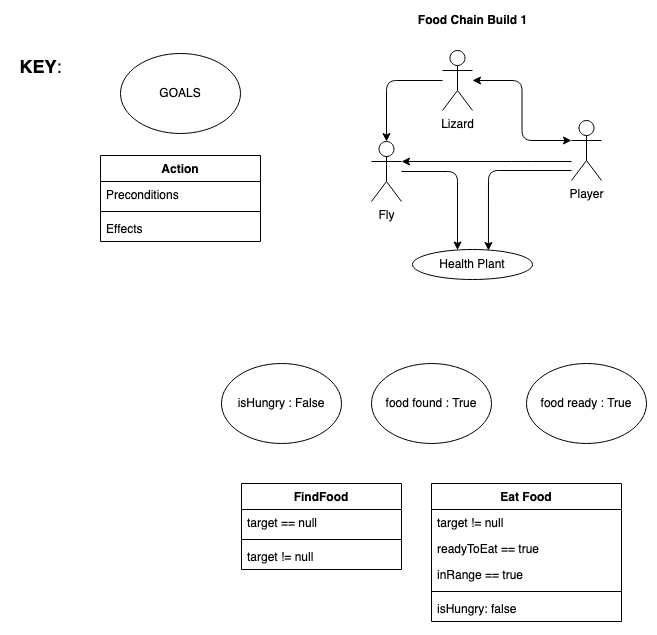
\includegraphics[width = 10cm ]{Actions and food chain build 1.png}}
    \caption{Goals and Actions with Food Chain}
\end{figure}

\subsection{Class Diagram}

\begin{figure}[H]
    \centering
    \fbox{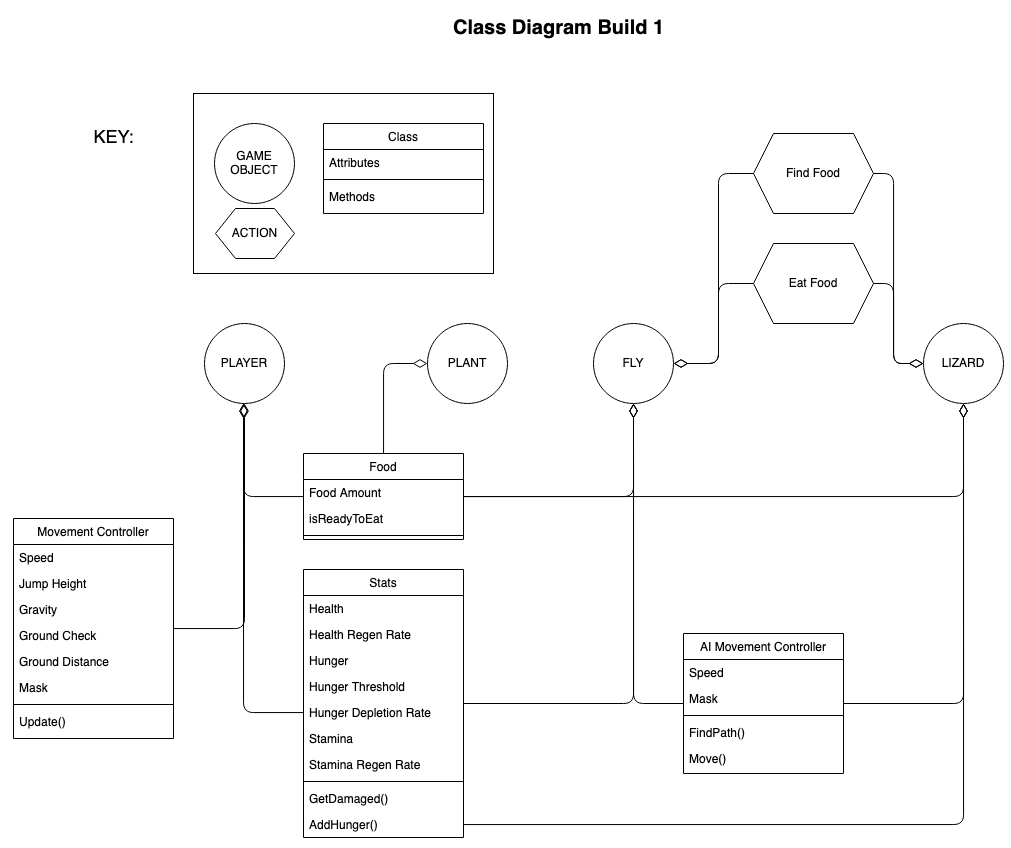
\includegraphics[width = 14.5cm ]{ClassDiagramBuild 1.png}}
    \caption{Class Diagram build 1}
\end{figure}

As explained before, Unity uses the Entity Component Paradigm of software design, the Circles represent Game Objects which are the entities in our game scene, and there are classes attached to them using compositional relationships, as you can se, one class is being used multiple times, and due to the lack of inheritance, there is very little interdependency. 
The Actions are represented by hexagons as at that moment in time, the decision had not been made on how the AI will be implemented.

% The Food Chain game object is unique in that there is only one required in a scene, and the Find Food action will access it to find out what the state of the food chain is to find food that is appropriate to that creature. The circle's are important game objects in the main Unity Scene, and they will be able to access each other.
\subsection{Creatures and AI}
I did extensive reading through the FEAR SDK\cite{fearSDK} that contains the full AI source code to fully understand the implementation of GOAP.
I also read up on many other implementations of GOAP and all of them are done in a very similar way with only minor structural differences. 
Peter Klooster created a multi-threaded GOAP System for Unity3D which he originally used in his game Basher Beatdown \cite{basherGoap}. This is a pretty simple implementation that includes a visualiser for the system as well.
Anne from the YouTube channel TheHappieCat did a GOAP implementation in Unity \cite{happieGoapVideo} based on the papers by Jeff Orkin and an article by Brent Owens \cite{brentOwensGoap} (taking the core system from here). She made a very informative video on the topic as well as walking through the code with a live simple example.
On Jeff Orkin's website, there was a reference to ReGOAP by Luciano Ferraro, which is a very generic C\# GOAP library, that was used in Unity3D, but can be used anywhere. Compared to the other implementations, this has been officially released on the Unity Asset store, however the code seems to be quite verbose and is not well commented, giving me a hard time understanding how to use it.

Based on all this I started creating my own GOAP system, however, it became very time consuming to create, and based on the gannt chart I had made, I was running behind on schedule; as the main focus of the project is to create the interaction between these different AI agents, and not the core AI system itself, I decided to use the implementation provided by Brent Owens \cite{brentOwensGoapCode} which is under the MIT licence. This is a very bare bones implementation only consisting of 6 scripts, and with the video explanation by TheHappieCat this was the simplest one I could implement and still have a great amount of flexibility in modifying the code due to its loosely coupled nature.

After I landed on this implementation of GOAP, I decided to start modelling out the different actions (with their preconditions and effects (post-conditions)), different creatures with their world state and the list of goals they would like to achieve. As Unity works with game objects made up of components, I decided to plan out the agents in an unconventional manner before creating the class diagrams. 

As can be seen in the UI figure, the meshes for the creatures were kept simple to ensure that the AI system worked, the movement system was also a trivial direct transformation towards the target for the same reason.

To add GOAP AI behaviour to an Agent, a script had to be attached that implemented the \lstinline{IGoap} interface provided by Brent Owens, and then have the \lstinline{GoapAgent} script attached which uses the \lstinline{GoapPlanner}. Now actions (inherited from \lstinline{GoapAction}) can be attached as scripts to the game object and the planner will automatically consider them. The script that inherits \lstinline{IGoap} will contain the world state and the desired goal state. The \lstinline{GoapAction}s will contain their own \textbf{preconditions} and \textbf{effects} and a \textbf{procedural precondition} method that the planner will consider when choosing the plan of action.

\begin{lstlisting}[language=c]
// inside Creatures : IGoap 
// world state
worldData.Add(new KeyValuePair<string, object>("isHungry", (hunger < hungerThreshold)));
// goal
goal.Add(new KeyValuePair<string, object>("isHungry", false));

// For Lizard that inherits creature
worldData.Add(new KeyValuePair<string, object>("damagePlayer", false)); 
goal.Add(new KeyValuePair<string, object>("damagePlayer", true));
 
// inside ActionEatFood.cs
addPrecondition("isHungry", true);
addEffect("isHungry", false);
cost = 1f;
\end{lstlisting}

This build of the Ai was functional however had a few issues. The Lizard enemy would only choose the player and not the fly, and it would eat anything. A food chain was added in the main build to fix this.

\subsection{Weapon}
For the melee weapon for the player to attack with, a pre-made sword asset was used (please refer to the asset listing) which was then imported into blender and 4 animation states were created. 

First the model was rigged using one bone, starting from the hilt of the sword. Then 4 different animations were created using key-framing and Blender's Dope Sheet editor, the idle animation and Attack 1 lasted 30 frames each and the Attack 2 and 3 lasted 20 frames each. This was then exported as an FBX file, which supports animations and textures to be baked into it and imported into Unity.
\begin{figure}[H]
    \begin{minipage}{.2\textwidth}
        \centering
        \fbox{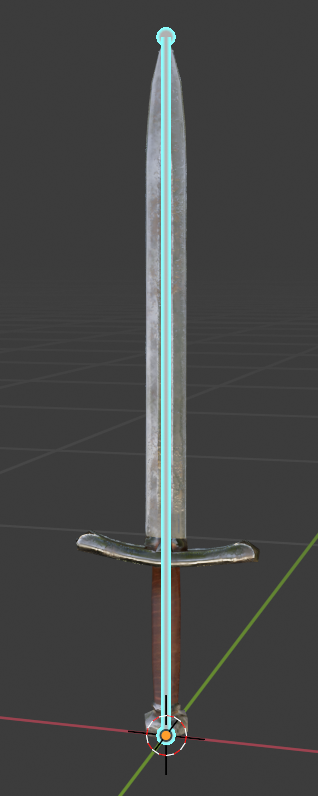
\includegraphics[width = 2cm ]{SwordBone.png}}
        \caption{Sword model rigged with a single bone}
    \end{minipage}
    \begin{minipage}{.8\textwidth}
        \centering
        \fbox{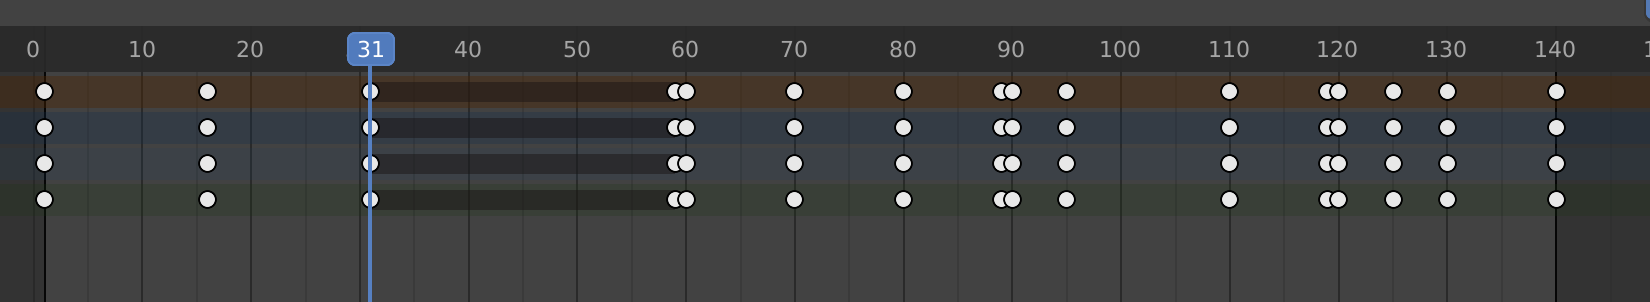
\includegraphics[width = 10cm ]{SwordKeyframes.png}}
        \caption{Dope sheet/Key-frames for 4 animations in Blender}
    \end{minipage}
\end{figure}

When importing it into Unity, the animations had to be split up into to 4 different actions as currently they were all done on one track (this was taken note of and the animations for the creatures were created on different tracks withing Blender, allowing an easier import process). In the heirarchy the sword was attached to an Empty called LeftHand to place it in the correct position, and this was parented under the Main Camera, making it so that the sword's transformation follows where the player is looking.

\begin{figure}[H]
    \begin{minipage}{.5\textwidth}
        \centering
        \fbox{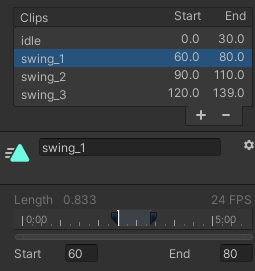
\includegraphics[width = 5cm ]{Sword_Unity_Animation_Import_Split.png}}
        \caption{Splitting Animations up for the Sword}
    \end{minipage}
    \begin{minipage}{.5\textwidth}
        \centering
        \fbox{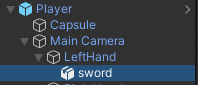
\includegraphics[width = 5cm ]{Sword_Unity_Heirarchy.png}}
        \caption{Sword in the Unity Hierarchy view}
    \end{minipage}
\end{figure}

An animation controller had to be created to switch between the different animations and create a combo system so a single click will only lead to the first swing, however clicking more than once will add the clicks to a buffer then swing the sword the appropriate number of times.

A tutorial by GRIMOIRE \cite{comboSystem} was used to understand how to do this inside of Unity and its animation system and implemented it in a similar manner.

\begin{figure}[H]
    \centering
    \fbox{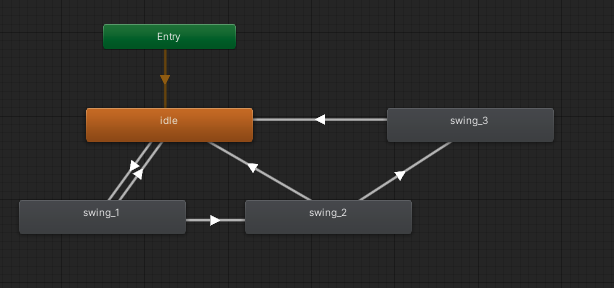
\includegraphics[width = 10cm ]{Sword_Animator.png}}
    \caption{Animation Controller attached to the Sword}
\end{figure}


\subsection{UI}
For the UI of the game, a decision was made to go without a main menu screen as there is only one level showcasing the use of the AI. 

The first UI designed was for the Creature displaying the stats above their meshes in game. This is one of the spacial UI elements in the game. Below is the initial sketch created in Adobe Illustrator.

\begin{figure}[H]
    \centering
    \fbox{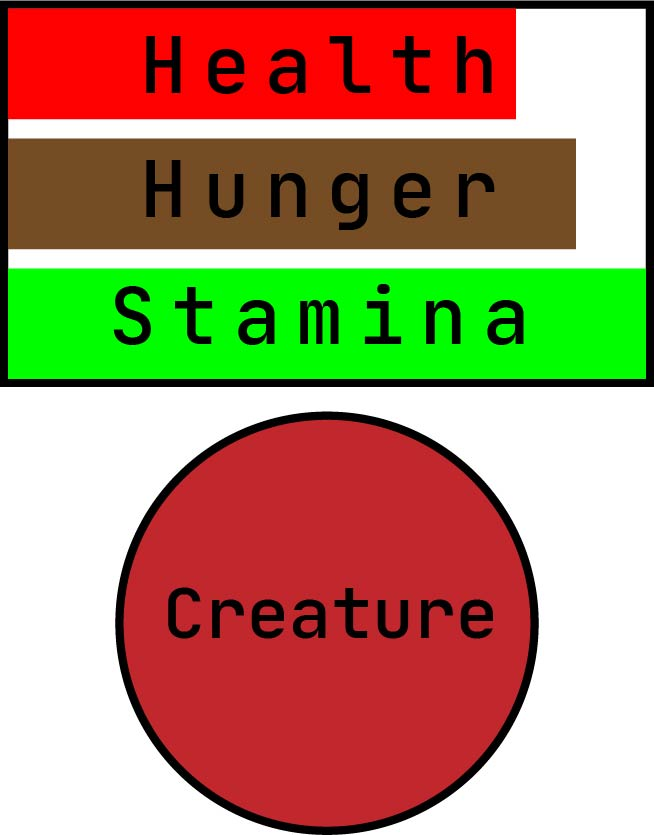
\includegraphics[width = 7cm ]{Stats_UI.jpg}}
    \caption{Creature UI Sketch}
\end{figure}

In Unity this was done by creating a canvas with multiple image sprites, these image sprites have a fill amount that goes from 0 to 1 which can be easily interpolated between by dividing the current values of the stat by their max value.

\begin{figure}[H]
    \begin{minipage}{.5\textwidth}
        \centering
        \fbox{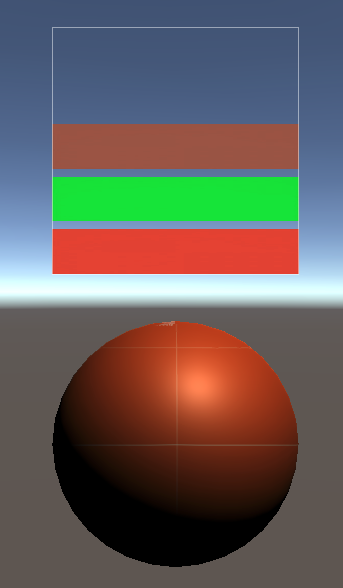
\includegraphics[width = 5cm ]{Stats_UI_Build1.png}}
        \caption{Creature UI in Unity}
    \end{minipage}
    \begin{minipage}{.5\textwidth}
        \centering
        \fbox{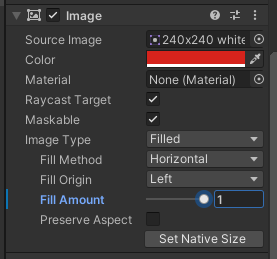
\includegraphics[width = 5cm ]{Unity_Image_Panel.png}}
        \caption{Image Component in Unity}
    \end{minipage}
\end{figure}

This canvas is parented to the Creature and the position is offset on the Y axis, so its transformation will follow its parent.

A script was created to manage the fill amounts, this was done by accessing a reference to the stats component in the parent object and then calculating the fill amount from there (see code snippet below).

\begin{lstlisting}[language=c]
void FixedUpdate() {
        healthBar.fillAmount = creatureStats.GetHealth() / 100;
        staminaBar.fillAmount = creatureStats.GetStamina() / 100;
        hungerBar.fillAmount = creatureStats.GetHunger() / 100;
        hungerThresholdBar.fillAmount = creatureStats.GetHungerThreshold() / 100;
}
\end{lstlisting}

\subsection{Unity Project}

Below is what the first version of the Unity scene looked like after adding the sword and basic AI components in.

\begin{figure}[H]
    \centering
    \fbox{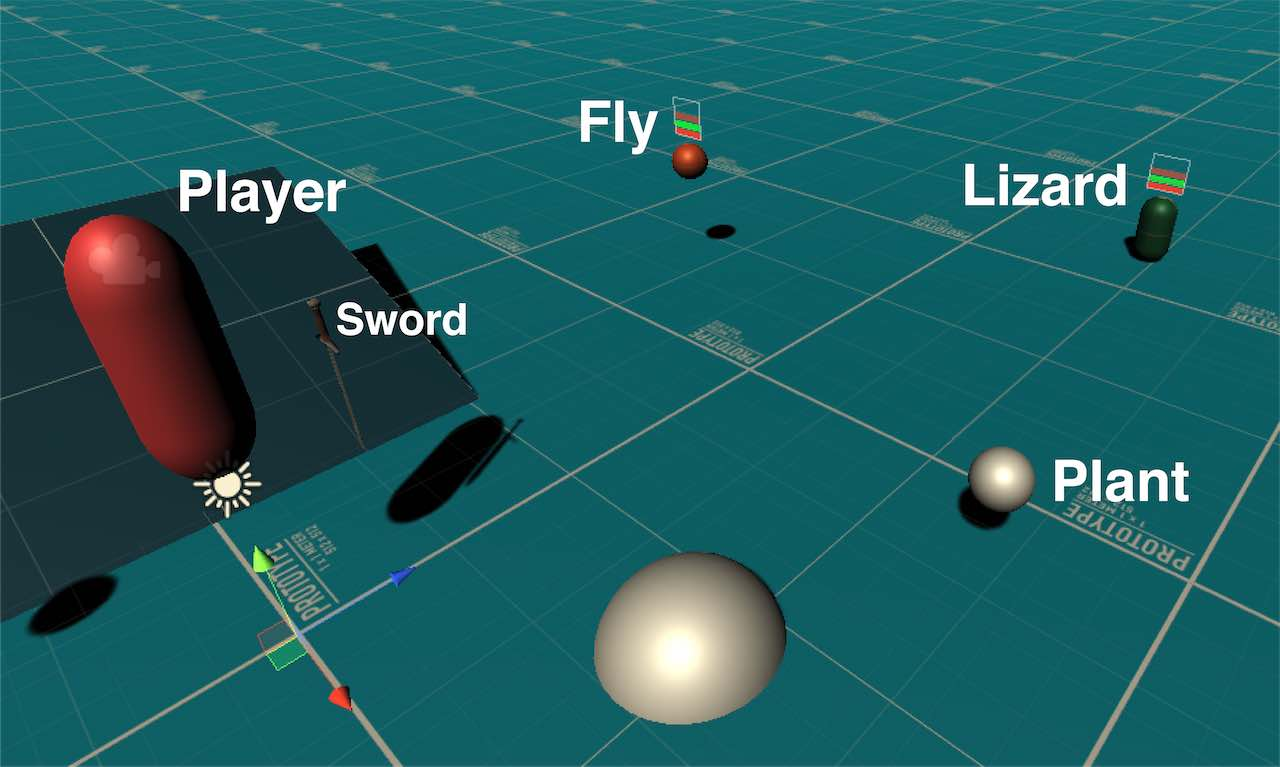
\includegraphics[width = 15cm]{Unity_Scene_Build_1_annotated.jpg}}
    \caption{Annotated view of Unity Scene}
\end{figure}


\section{Main Product}
\subsection{Creatures and AI}
The meshes of the creatures were changed; a set of animated ice age animal meshes by Riley on itch.io (please see in the asset listing). These were aesthetically pleasing while having a low poly count keeping the file size and performance overhead to a minimum. 

The saber-tooth (replacing the lizard in the food chain) had 4 animation states, of which only 3 were required, however the sloth (replacing the fly in the food chain) only had 2 animation states, walk and idle, an additional one for biting was required for when it eats food. 

The model was imported into Blender, however the model seemed to have an unnecessary number of bones, most of which did not have an effect to the model. Seeing this, the model had to be rigged again and freshly animated. The same process was used as the sword but with a higher complexity.

\begin{figure}[H]
    \begin{minipage}{.5\textwidth}
        \centering
        \fbox{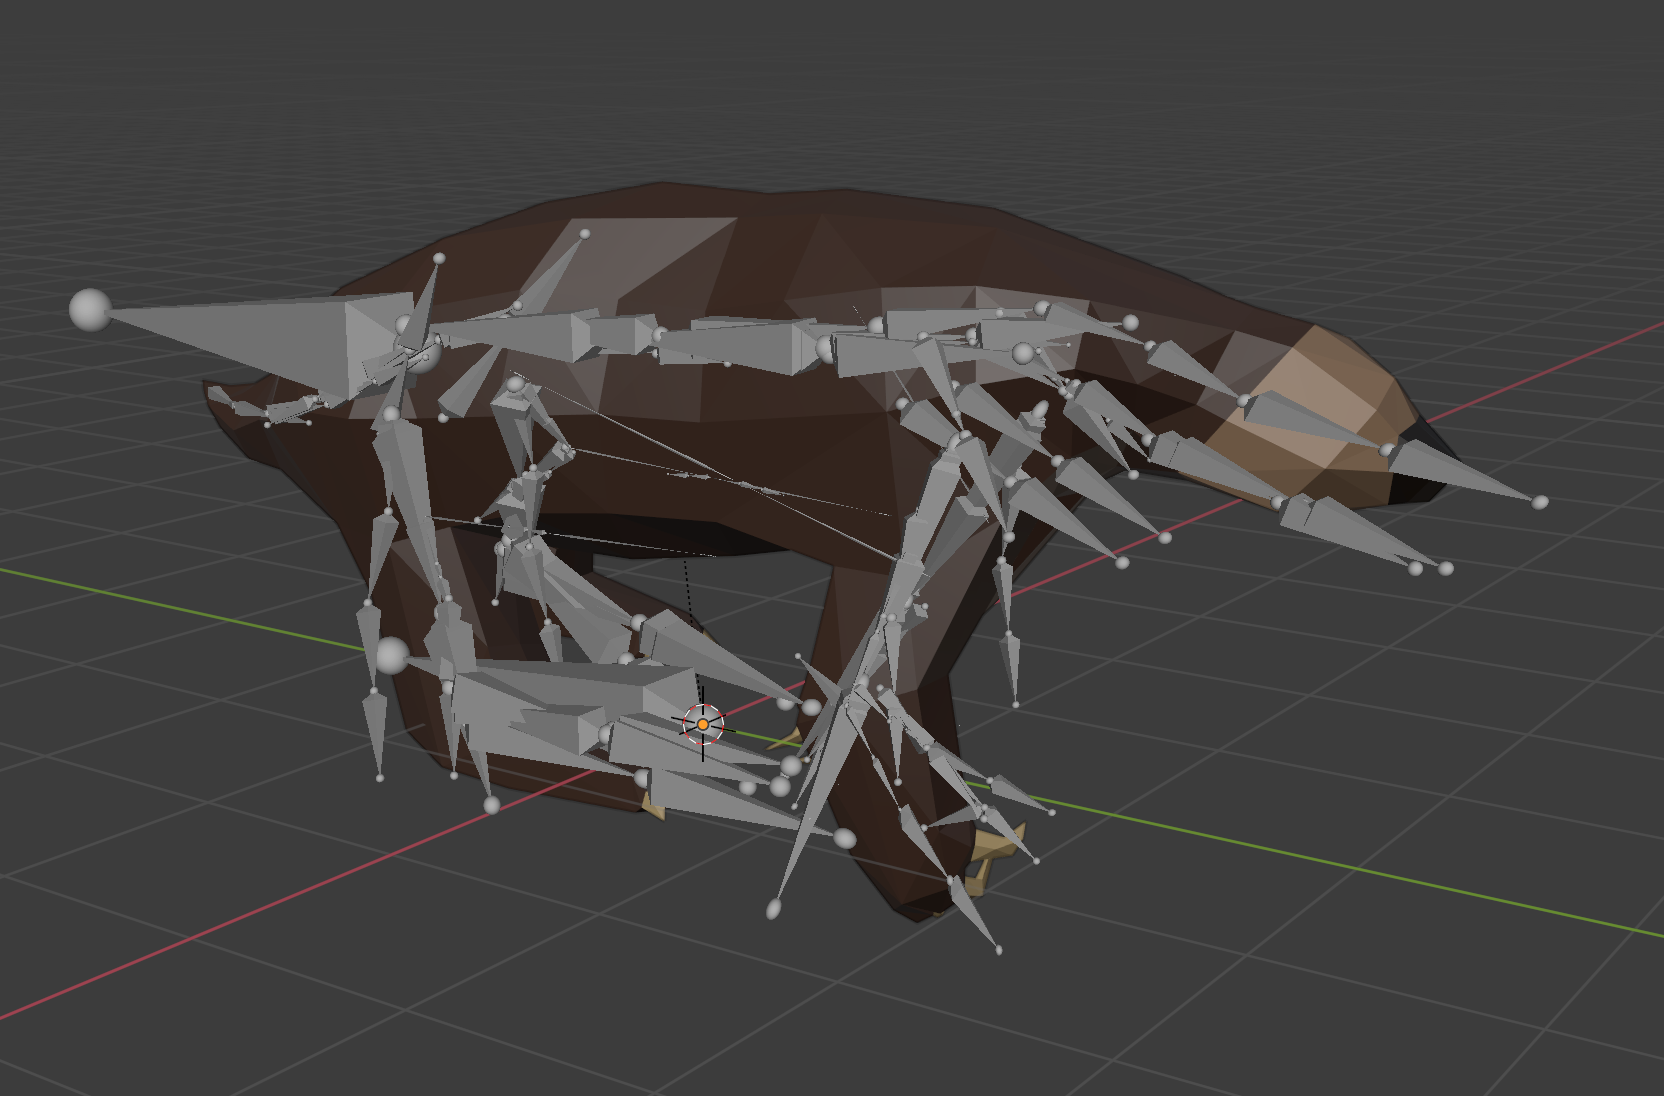
\includegraphics[width = 7cm ]{Sloth_Model_Messy_Rig.png}}
        \caption{Messy Original Sloth Rig}
    \end{minipage}
    \begin{minipage}{.5\textwidth}
        \centering
        \fbox{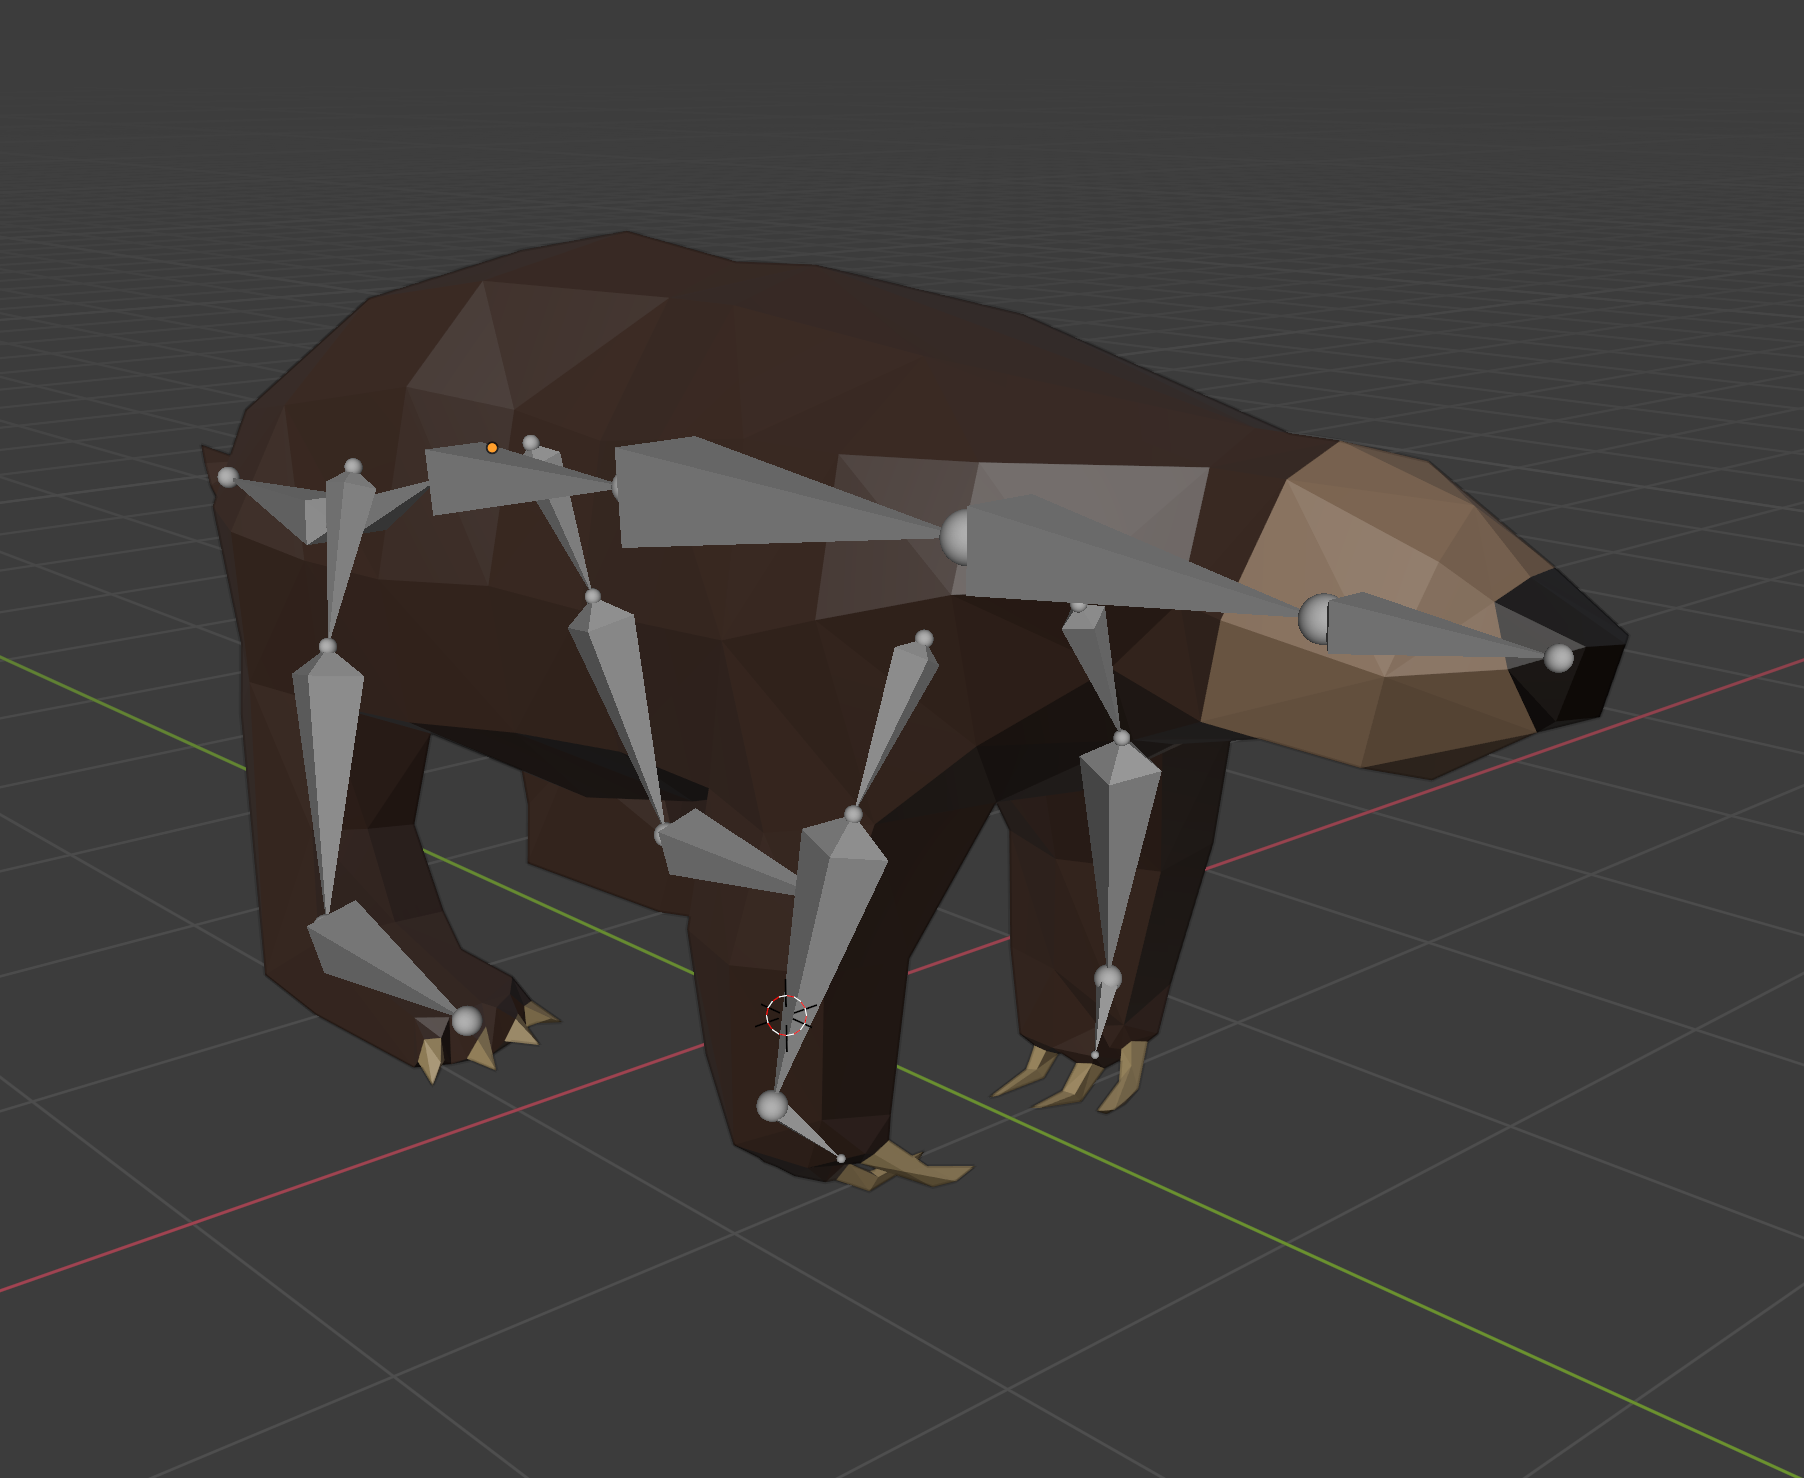
\includegraphics[width = 7cm ]{Sloth_Model_Clean_Rig.png}}
        \caption{Clean New Sloth Rig}
    \end{minipage}
\end{figure}

A path finding system was added in to facilitate better movement for the AI Agents. A* Pathfinding Project by Aron Granberg (see asset listings). This is a very nice and free library that provides the generation of many different type of nav meshes, the one used in the game is a Grid Graph

\chapter{Asset Listing}

\begin{thebibliography}{}
    \bibitem{doom93}
    id Software, id Software, (1993). DOOM. [computer game]. \\Available at: \url{https://store.bethesda.net/store/bethesda/en_IE/pd/productID.5361563100/currency.GBP}
    \bibitem{farcry}
    Ubisoft.com. 2021. Far Cry franchise. [online] Available at: \url{https://www.ubisoft.com/en-gb/franchise/far-cry/} [Accessed 9 February 2021].
    \bibitem{farCryPrimalCompanions}
    Thompson, T., 2018. Primal Instinct | Companion AI in Far Cry Primal. [online] Gamasutra.com. Available at: \url{https://gamasutra.com/blogs/TommyThompson/20180906/325967/Primal_Instinct__Companion_AI_in_Far_Cry_Primal.php} [Accessed 12 February 2021].
    \bibitem{emergentGameplay}
    "Le Gameplay emergent (in French)". jeuxvideo.com. 2006-01-19. Available at: \url{https://www.jeuxvideo.com/dossiers/00006203/le-gameplay-emergent.htm} [Accessed 9th February 2021]
    \bibitem{gameAiByExample}
    Buckland, M., 2010. Programming Game AI by Example. Burlington: Jones \& Bartlett Learning, LLC, p.46.
    \bibitem{halo2}
    Bungie, Microsoft Game Studios. Halo 2 [computer game]. 04/09/2004.
    \bibitem{behaviourTrees}
    Simpson, C., 2014. Behavior trees for AI: How they work. [online] Gamasutra.com. Available at: \url{https://www.gamasutra.com/blogs/ChrisSimpson/20140717/221339/Behavior_trees_for_AI_How_they_work.php} [Accessed 12 February 2021].
    \bibitem{goap}
    Orkin, J., n.d. Goal-Oriented Action Planning (GOAP). [online] \\Alumni.media.mit.edu. Available at: \url{http://alumni.media.mit.edu/~jorkin/goap.html} [Accessed 12 February 2021].
    \bibitem{applyingGoap}
    Orkin, J., n.d. Applying Goal-Oriented Action Planning to Games. [online] \\Alumni.media.mit.edu. Available at: \url{http://alumni.media.mit.edu/~jorkin/GOAP_draft_AIWisdom2_2003.pdf} [Accessed 12 February 2021].
    \bibitem{goapTommyTompson}
    Thompson, T., 2020. Building the AI of F.E.A.R. with Goal Oriented Action Planning. [online] Gamasutra.com. Available at: \url{https://www.gamasutra.com/blogs/TommyThompson/20200507/362417/Building_the_AI_of_FEAR_with_Goal_Oriented_Action_Planning.php} [Accessed 13 February 2021].
    \bibitem{fearSDK}
    Monolith Productions, Inc., 2004, Fear SDK 1.08 [code] Available at: \url{http://fear.filefront.com/file/FEAR_v108_SDK;71433} and \url{https://github.com/xfw5/Fear-SDK-1.08.git}
    \bibitem{basherGoap}
    Klooster, Peter, GOAP, a multi-threaded library for Unity [code] Available at: \url{https://github.com/crashkonijn/GOAP}, under Apache-2.0 licence
    \bibitem{happieGoapVideo}
    Anne, 2016. Combat AI for Action-Adventure Games Tutorial [Unity/C\#] [GOAP]. [video] Available at: \url{https://youtu.be/n6vn7d5R_2c} [Accessed 13 February 2021].
    \bibitem{brentOwensGoap}
    Owens, B., 2014. Goal Oriented Action Planning for a Smarter AI. [online] Game Development Envato Tuts+. Available at: \url{https://gamedevelopment.tutsplus.com/tutorials/goal-oriented-action-planning-for-a-smarter-ai--cms-20793} [Accessed 13 February 2021].
    \bibitem{brentOwensGoapCode}
    Owens, B., 2014. Goal Oriented Action Planning for a Smarter AI. [code]. Available at: \url{https://github.com/sploreg/goap} [Accessed 13 February 2021].
    \bibitem{drawIo}
    App.diagrams.net. 2021. Flowchart Maker \& Online Diagram Software. [online] Available at: \url{https://app.diagrams.net/} [Accessed 20 February 2021].
    \bibitem{codingPractices}
    En.wikipedia.org. n.d. Coding best practices - Wikipedia. [online] Available at: \url{https://en.wikipedia.org/wiki/Coding_best_practices} [Accessed 15 April 2021].
    \bibitem{CompOverInherit}
    Youtu.be. 2021. Composition over Inheritance. [online] Available at: \url{https://youtu.be/wfMtDGfHWpA} [Accessed 15 April 2021].
    \bibitem{UIChoices}
    F, J., 2021. What Are Your UI Choices. [online] Medium. Available at: \url{https://medium.com/@gfruity/what-are-your-ui-choices-834ea7d937c} [Accessed 18 April 2021].
    \bibitem{comboSystem}
    Grimoirehex.com. 2017. Unity 3D – Combo System Animation – GRIMOIRE. [online] Available at: \url{https://www.grimoirehex.com/unity-3d-combo-animation/} [Accessed 15 February 2021].
\end{thebibliography}
\end{document}